\begin{figure}[!hbtp]
  \centering  % \vspace{-0.3 cm}
  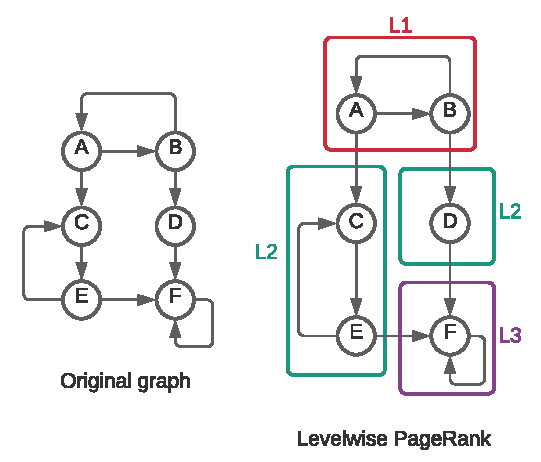
\includegraphics[width=0.48\textwidth]{out/about-levelwise.pdf}
  \caption{Consider a graph with 6 vertices, as shown on the left. This graph has 4 SCCs, C1 with vertices A and B, C2 with vertices C and E, C3 with vertex D, and C4 with vertex F. Its block-graph consists of vertex C1 pointing to C2, which then points to C3. This is the order in which SCCs are processed as per the \levelwisePR{} algorithm.}
  \label{fig:levelwise}
\end{figure}
